\documentclass{beamer}
 
\usepackage[utf8]{inputenc}

\usetheme{Szeged}
\usecolortheme{beaver} 
 

\title{Lerntraining Software}
\subtitle{Python}
\author{Sophie Aerdker}
\institute{Ruhr-Universit\"at Bochum}
\date{Mai 2018}
 
 
 
\begin{document}
 
\frame{\titlepage}
\begin{frame}
\frametitle{Table of Contents}
	\tableofcontents
\end{frame}

\section{Overview}

\begin{frame}
\frametitle{Overview}
	Python is ...\\
	\begin{itemize}
		\item interpreted 
		\item interactive 
		\item object-oriented 
		\item a beginners language!
	\end{itemize}
\end{frame}

\subsection{Setup}

\begin{frame}
\frametitle{For you at home, here \texttt{python} is already installed!}
	\begin{itemize}
		\item Check if \texttt{Python} is already installed: open a terminal and type "python"
		\item Linux:
		\item Windows:
	\end{itemize}
	Using \textit{Anaconda}:
	\begin{itemize}
		\item Linux:
		\item Windows:
	\end{itemize}
	Or use an IDE like \textit{eclipse} or \textit{Visual Studio}
\end{frame}

\section{First Steps}
\subsection{Hello World!}

\begin{frame}
\frametitle{ Hello World!}
	\begin{columns}[T]
		\begin{column}[T]{7cm}
			\begin{itemize}
				\item open an editor 
				\item type: \texttt{print "Hello World!"}
				\item save it as "HelloWorld.py" under ...
				\item open a terminal and go to your directory with cd ...
				\item type: \texttt{python HelloWorld.py}
			\end{itemize}
		\end{column}
		\begin{column}[T]{5cm}
			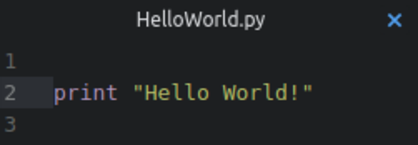
\includegraphics[width = 1\textwidth]{HelloWorld.pdf}
		\end{column}
	\end{columns}
\end{frame}

\subsection{Simple Calculations}

\begin{frame}
\frametitle{Simple Calculations}
	\begin{columns}[T]
		\begin{column}[T]{7cm}
			\begin{itemize}
				\item now type e.g. \texttt{x = 5} and \texttt{y = 10} under your print statement
				\item type \texttt{print} and a calculation using +,-,*,/
				\item save the file, go to your terminal and type \texttt{python HelloWorld.py} or press $\uparrow$
				\item What is the result of \texttt{x/y}?
			\end{itemize}
		\end{column}
		\begin{column}[T]{3cm}
			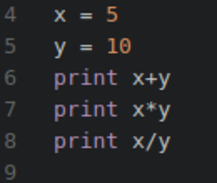
\includegraphics[width = 1\textwidth]{SimpleCalculations.pdf}
		\end{column}
	\end{columns}
\end{frame}

\section{Variable Types}

\begin{frame}
\frametitle{Variable Types}
	Python has five basic data types:
	\begin{itemize}
		\item Numbers, like 5 and 10
		\item Strings, like "Hello World!"
		\item Lists
		\item Dictionary
		\item Tuple
	\end{itemize}
	Data types can be stored in variables:
	\begin{itemize}
		\item  \texttt{x = 10}
		\item  \texttt{gravConstant = 9.81}
		\item  \texttt{s = "Hello World!"}
		\item  \texttt{name = "Sophie"}
	\end{itemize}
\end{frame}

\subsection{Numbers}

\begin{frame}
\frametitle{Basic numerical types with some examples}
	\begin{tabular}{c|c|c}
		Type & Examples & Comment \\ \hline
		int  & 3, -42 &  signed integer $ \leq 2,147,483,647$\\
		long & 51924361L & signed integer $>2,147,483,647$ \\
		float & 3.14, 3.0+e10, 0. & floating point real values \\
		complex & 42.0j, 2.+0.3j & complex numbers, imaginary unit j
 	\end{tabular}
 	
 	\begin{alertblock}{Integer Division}
 		The statement \texttt{5/10} is interpreted as an integer! Thus, its integer division is 0. Instead type 			\texttt{5./10.} to obtain a float-type value.
 	\end{alertblock}
 	\begin{block}{Boolean}
 		The result of a comparison which is \texttt{True} or \texttt{False} is called Boolean. \texttt{True} and 			\texttt{False} are special versions of 1 (or any non-zero/null value) and 0, respectively. You can use them in arithmetic contexts.
 	\end{block}	
\end{frame}

\subsection{Operators}

\begin{frame}
\frametitle{Arithmetic and Comparison Operators}
	\begin{tabular}{cc|c}
		\multicolumn{2}{c|}{Operator} & Examples  \\ \hline
		+ & Addition & 5+10 = 15  \\
		- & Subtraction & 10-5 = 5  \\
		* & Multiplication & 10*5 = 50   \\
		/ & Division & 10/5 = 2, 5/10 = 0, 5./10. = 0.5 \\
		** & Power & 10**5 = 10,000 \\
		\% & Modulus & 10\%5 = 0, 5\%10 = 5 \\
		// & Floor Division & 9.//2. = 4.0 \\ \hline
		== & equal & 5==10 is False, 5==5 is True  \\
		!= & not equal & 5!=10 is True, 5!=5 is False  \\
		$>$ & greater than & 10 $>$ 5 is True  \\
		$<$ & less than & 10 $<$ 5 is False \\
		\multicolumn{2}{l|}{$<=$ or $>=$} & 10 $>=$ 5 is True, 5 $<=$ 5 is True \\
 	\end{tabular}	
\end{frame}

\begin{frame}
\frametitle{Asignment Operators}
	\begin{tabular}{c|p{5cm}|p{3cm}}
		Operator & Description & Example  \\ \hline
		= & Assigns values from the right side to the left side & x = 5+10 \\
		+= & Adds right operand to the left one AND assigns the result to the left operand & x += 1 is equivalent to x = x + 1 \\ \hline	
		-= &  \multicolumn{2}{c}{x -= 1  is equivalent to x = x-1} \\
		*= &  \multicolumn{2}{c}{x *= 2 is equivalent to x = x*2} \\
		/= &  \multicolumn{2}{c}{x /= 2 is equivalent to x = x/2 }\\
		**= & \multicolumn{2}{c}{x **= 2 is equivalent to x = x**2} \\
		\%= &  \multicolumn{2}{c}{x \%= 2 is equivalent to x = x\%2 }\\
		//= &  \multicolumn{2}{c}{x //= 2 is equivalent to x = x//2 }\\ 	
 	\end{tabular}	
\end{frame}

\begin{frame}
\frametitle{Other Operators}
	\begin{alertblock}{Bitwise operators} 
		which perform bit by bit operations like binary AND, binary OR or shifting
	\end{alertblock}
	\begin{alertblock}{Logical operators} 
		\texttt{not} , \texttt{or} , \texttt{and} \\
	\end{alertblock}
	\begin{alertblock} {Membership operators} 
		\texttt{in} and \texttt{not in} \\test the membership in a \textit{sequence} such as lists or strings
	\end{alertblock}
	\begin{alertblock}{Identity operators} 
		\texttt{is} and \texttt{is not} \\compare the memory locations of two objects, you can often use them like \texttt{==} and \texttt{!=}	for example in \textit{if-statements}
	\end{alertblock}
\end{frame}

\section{Decision Making}

\begin{frame}
\frametitle{If-statements}
	\begin{columns}[T]
	\begin{column}[T]{5cm}
			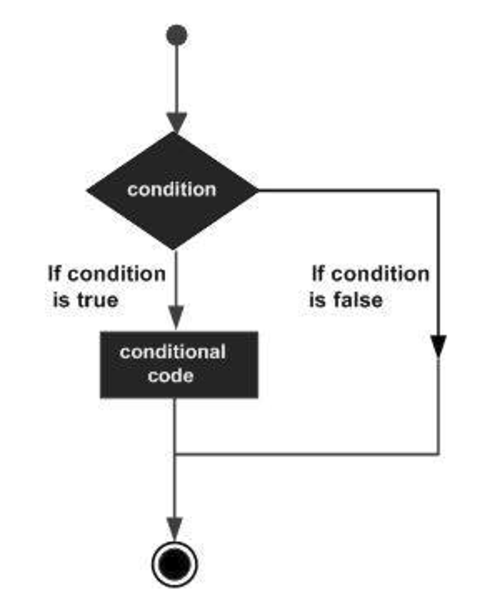
\includegraphics[width = 1\textwidth]{DecisionMaking.pdf}
		\end{column}
		\begin{column}[T]{3cm}
			use \texttt{if} and \texttt{else} conditions to execute a specific code if a condition is TRUE or to jump to the next (or another conditional) code otherwise	
		\end{column}	
	\end{columns}
\end{frame}

\begin{frame}
\frametitle{Example}
	\begin{columns}[T]
		\begin{column}[T]{0.6\textwidth}
			Some \texttt{if}, \texttt{elif}, \texttt{else} statements to compare the values x and y:\\
			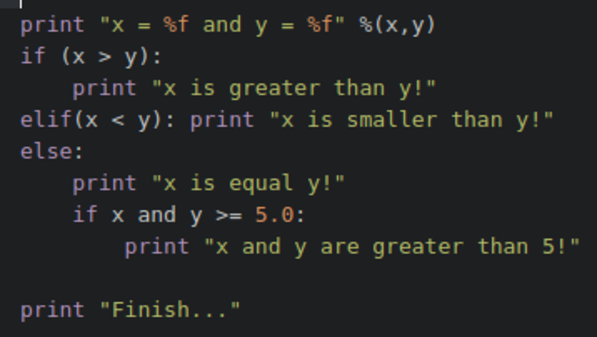
\includegraphics[width = 1\textwidth]{Comparison.pdf}
		\end{column}
		\begin{column}[T]{0.4\textwidth}
			Output for different values of x and y:\\
			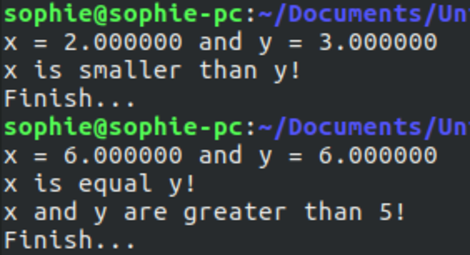
\includegraphics[width = 1\textwidth]{OutputComparison.pdf}	
		\end{column}	
	\end{columns}
	\begin{alertblock} {Syntax} 
		The conditional code has to be intended or stands in a line (only possible for one statement) with the condition. IDEs and many editors do this automatically.
	\end{alertblock}
\end{frame}

\begin{frame}
\frametitle{Exercises}
	\begin{itemize}
		\item Write the program \texttt{EvenOdd.py} which returns wether a variable is even or odd! \\ Use operators and condition statements and print the value as well as the result!
		\item Write the program \texttt{CharInString.py} which returns wether the string \texttt{"Hello World!"} contains a specific letter (a so called char)! \\ Use membership operators and the program should be case sensitive to keep it simple.
	\end{itemize}
	
\end{frame}


\end{document}